\def\pgfsysdriver{pgfsys-dvipdfm.def}
\pdfpagewidth=\paperwidth
\pdfpageheight=\paperheight

\documentclass[12pt]{beamer}
\usetheme{Warsaw}

\usepackage{color}
\usepackage{xcolor,colortbl}
\usepackage{indentfirst}
\usepackage[export]{adjustbox}
\usepackage{float}
\usepackage{wrapfig}
\usepackage{setspace}
\usepackage{fontspec}
\usepackage{graphicx}
\usepackage{subcaption}
\usepackage{pgfpages}
\usepackage{amsmath}
\usepackage{bbm}
\usepackage{bm}
\usepackage{dsfont}
\usepackage{xeCJK}
\usepackage[backend=biber]{biblatex}

%\setbeamertemplate{footline}{}
\setbeamertemplate{headline}{}
\setbeamertemplate{navigation symbols}{}
%\setbeameroption{show notes on second screen=right}
\setbeamertemplate{note page}[plain]

\addtobeamertemplate{frametitle}{\vspace*{-5pt}}{\vspace*{0pt}}
\setbeamertemplate{section in toc shaded}[default][70]
\setbeamertemplate{subsection in toc shaded}[default][70]

\renewcommand*{\thefootnote}{[\arabic{footnote}]}

\usefonttheme{professionalfonts}

\setsansfont{Open Sans}[Scale=0.75]
\setCJKsansfont[Scale=0.75]{WenQuanYi Micro Hei}

\setbeamerfont{title}{ size={\fontsize{16}{16}} }
%\setbeamerfont{date}{ size={\fontsize{20}{20}} }
\setbeamerfont{note page}{	size={\fontsize{14}{16.8}} }
%\setbeamerfont{note title}{ size = {\fontsize{12}{12}} }
\setbeamerfont{institute}{ size={\fontsize{10}{10}} }
\setbeamerfont{footnote}{ size={\fontsize{9}{9}} }
\setbeamerfont{footline}{ size={\fontsize{7}{7}} }
\setbeamerfont{author}{ size={\fontsize{12}{12}} }
\setbeamerfont{date}{ size={\fontsize{12}{12}} }

\def\dr{\mathrm{d}}

\def\pleq{\preccurlyeq}
\def\pgeq{\succcurlyeq}
\def\pge{\succ}
\def\ple{\prec}

\def\Approx#1{\approx_{#1}}

\def\Span#1{\textbf{Span}\left(#1  \right)}
\def\bvec#1{{\mbox{\boldmath $#1$}}}


\def\prob#1#2{\mbox{Pr}_{#1}\left[ #2 \right]}
\def\pvec#1#2{\vec{\mbox{P}}^{#1}\left[ #2 \right]}
\def\expec#1#2{{\mathbb{E}}_{#1}\left[ #2 \right]}
\def\var#1{\mbox{\bf Var}\left[ #1 \right]}
\newcommand{\E}{\mbox{{\bf E}}}

\def\defeq{\stackrel{\mathrm{def}}{=}}
\def\setof#1{\left\{#1  \right\}}
\def\sizeof#1{\left|#1  \right|}




\def\floor#1{\left\lfloor #1 \right\rfloor}
\def\ceil#1{\left\lceil #1 \right\rceil}

\def\dim#1{\mathrm{dim} (#1)}
\def\sgn#1{\mathrm{sgn} (#1)}

\def\union{\cup}
\def\intersect{\cap}
\def\Union{\bigcup}
\def\Intersect{\bigcap}

\def\eps{\epsilon}

\def\abs#1{\left|#1  \right|}

\def\trace#1{\mathrm{Tr} \left(#1 \right)}
\def\norm#1{\left\| #1 \right\|}
\def\smallnorm#1{\| #1 \|}


\def\calC{\mathcal{C}}
\def\calE{\mathcal{E}}
\def\calG{\mathcal{G}}
\def\calL{\mathcal{L}}
\def\calS{\mathcal{S}}


\newcommand\Ppsi{\boldsymbol{\mathit{\Psi}}}
\newcommand\PPsi{\boldsymbol{\mathit{\Psi}}}
\newcommand\ppsi{\boldsymbol{\mathit{\psi}}}
\newcommand\pphi{\boldsymbol{\mathit{\phi}}}
\newcommand\Llambda{\boldsymbol{\mathit{\Lambda}}}
\newcommand\PPi{\boldsymbol{\Pi}}

\newcommand\ppi{\boldsymbol{\pi}}
\newcommand\cchi{\boldsymbol{\chi}}
\newcommand\aalpha{\boldsymbol{\alpha}}
\newcommand\bbeta{\boldsymbol{\beta}}
\newcommand\ggamma{\boldsymbol{\gamma}}
\newcommand\ddelta{\boldsymbol{\delta}}

\newcommand\er{R_{\mathrm{eff}}}
\newcommand\ccc{C_{\mathrm{CC}}}
\newcommand\ci{C_{\mathrm{I}}}


\def\aa{\pmb{\mathit{a}}}
\newcommand\bb{\boldsymbol{\mathit{b}}}
\newcommand\cc{\boldsymbol{\mathit{c}}}
\newcommand\dd{\boldsymbol{\mathit{d}}}
\newcommand\ee{\boldsymbol{\mathit{e}}}
\newcommand\ff{\boldsymbol{\mathit{f}}}
\renewcommand\gg{\boldsymbol{\mathit{g}}}
\newcommand\ii{\boldsymbol{\mathit{i}}}
\newcommand\jj{\boldsymbol{\mathit{j}}}
\newcommand\kk{\boldsymbol{\mathit{k}}}
\renewcommand\ll{\boldsymbol{\mathit{l}}}
\newcommand\pp{\boldsymbol{\mathit{p}}}
\newcommand\qq{\boldsymbol{\mathit{q}}}
\newcommand\bs{\boldsymbol{\mathit{s}}}
\newcommand\nn{\boldsymbol{\mathit{n}}}
\newcommand\rr{\boldsymbol{\mathit{r}}}
\renewcommand\ss{\boldsymbol{\mathit{s}}}
\def\tt{\boldsymbol{\mathit{t}}}
\newcommand\uu{\boldsymbol{\mathit{u}}}
\newcommand\vv{\boldsymbol{\mathit{v}}}
\newcommand\ww{\boldsymbol{\mathit{w}}}
\newcommand\yy{\boldsymbol{\mathit{y}}}
\newcommand\zz{\boldsymbol{\mathit{z}}}
\newcommand\xx{\boldsymbol{\mathit{x}}}
\newcommand\xxbar{\overline{\boldsymbol{\mathit{x}}}}

\renewcommand\AA{\boldsymbol{\mathit{A}}}
\newcommand\BB{\boldsymbol{\mathit{B}}}
\newcommand\CC{\boldsymbol{\mathit{C}}}
\newcommand\DD{\boldsymbol{\mathit{D}}}
\newcommand\EE{\boldsymbol{\mathit{E}}}
\newcommand\GG{\boldsymbol{\mathit{G}}}
\newcommand\II{\boldsymbol{\mathit{I}}}
\newcommand\JJ{\boldsymbol{\mathit{J}}}
\newcommand\KK{\boldsymbol{\mathit{K}}}
\newcommand\NN{\boldsymbol{\mathit{N}}}
\newcommand\MM{\boldsymbol{\mathit{M}}}
\newcommand\LL{\boldsymbol{\mathit{L}}}
\newcommand\PP{\boldsymbol{\mathit{P}}}
\newcommand\QQ{\boldsymbol{\mathit{Q}}}
\newcommand\RR{\boldsymbol{\mathit{R}}}
\renewcommand\SS{\boldsymbol{\mathit{S}}}
\newcommand\UU{\boldsymbol{\mathit{U}}}
\newcommand\WW{\boldsymbol{\mathit{W}}}
\newcommand\VV{\boldsymbol{\mathit{V}}}
\newcommand\XX{\boldsymbol{\mathit{X}}}
\newcommand\YY{\boldsymbol{\mathit{Y}}}



\newcommand\MMtil{\boldsymbol{\mathit{\tilde{M}}}}
\newcommand\AAtilde{\boldsymbol{\mathit{\tilde{A}}}}
\newcommand\LLtil{\boldsymbol{\mathit{\tilde{L}}}}
\newcommand\MMtilde{\boldsymbol{\mathit{\tilde{M}}}}

\newcommand\AAn{\boldsymbol{\mathcal{A}}}
\newcommand\ZZ{\boldsymbol{\mathit{Z}}}

\newcommand\AAhat{\boldsymbol{\widehat{\mathit{A}}}}
\newcommand\AAapprox{\boldsymbol{\widetilde{\mathit{A}}}}
\newcommand\DDhat{\boldsymbol{\widehat{\mathit{D}}}}
\newcommand\DDapprox{\boldsymbol{\widetilde{\mathit{D}}}}
\newcommand\LLhat{\boldsymbol{\widehat{\mathit{L}}}}
\newcommand\LLapprox{\boldsymbol{\widetilde{\mathit{L}}}}
\newcommand\MMhat{\boldsymbol{\widehat{\mathit{M}}}}
\newcommand\MMapprox{\boldsymbol{\widetilde{\mathit{M}}}}
\newcommand\ZZhat{\boldsymbol{\widehat{\mathit{Z}}}}

\newcommand\AAtil{\boldsymbol{\widetilde{\mathit{A}}}}
\newcommand\DDtil{\boldsymbol{\widetilde{\mathit{D}}}}


\newcommand\bbtil{\boldsymbol{\tilde{\mathit{b}}}}
\newcommand\xxtil{\boldsymbol{\tilde{\mathit{x}}}}


\newcommand\Otil{\widetilde{O}}

\newcommand\xhat{\boldsymbol{\hat{\mathit{x}}}}
\newcommand\uhat{{\hat{{u}}}}
\newcommand\vhat{{\hat{{v}}}}
\newcommand\what{{\hat{{w}}}}

\newcommand\Ghat{{\widehat{{G}}}}

\newcommand{\sym}[1]{\mathrm{sym} (#1)}

\newcommand{\one}{\mathbf{1}}
\newcommand{\diag}{\textsc{diag}}
\newcommand\LLs{\boldsymbol{\mathit{L}_s}}

\newcommand{\todo}[1]{{\bf \color{red} TODO: #1}}
\newcommand{\rp}[1]{{\bf \color{green} RP: #1}}
\newcommand{\hl}[1]{{\bf \color{green} HL: #1}}

\newcommand{\expct}[2]{\ensuremath{\mathop{\text{\normalfont \textbf{E}}}_{#1}}\left[#2\right]}

\DeclareMathOperator*{\argmin}{arg\,min}
\DeclareMathOperator*{\argmax}{arg\,max}

\newcommand{\kh}[1]{\left(#1\right)}

\newcommand{\bsk}{\backslash_\theta}

\definecolor{Gray}{gray}{0.95}
\definecolor{LightCyan}{rgb}{0.9,1,1}

\newcolumntype{a}{>{\columncolor{LightCyan}}c}
\newcolumntype{b}{>{\columncolor{Gray}}c}


%%%%%%%%%%%%%%%%%%%%%%%%%%%%%%%%%%%%%%%%%%%%%%%%%%%%%%%%%%%%%%%%%%%%%%%%%%%%%%%%%%%%%%%%%%%%%%%%%%%%%%%%%%%%%%%%%%%%%%%%
%%%%%%%%%%%%%%%%%%%%%%%%%%%%%%%%%%%%%%%%%%%%%%%%%%%%%%%%%%%%%%%%%%%%%%%%%%%%%%%%%%%%%%%%%%%%%%%%%%%%%%%%%%%%%%%%%%%%%%%%
%%%%%%%%%%%%%%%%%%%%%%%%%%%%%%%%%%%%%%%%%%%%%%%%%%%%%%%%%%%%%%%%%%%%%%%%%%%%%%%%%%%%%%%%%%%%%%%%%%%%%%%%%%%%%%%%%%%%%%%%
%%%%%%%%%%%%%%%%%%%%%%%%%%%%%%%%%%%%%%%%%%%%%%%%%%%%%%%%%%%%%%%%%%%%%%%%%%%%%%%%%%%%%%%%%%%%%%%%%%%%%%%%%%%%%%%%%%%%%%%%

\title[Kirchhoff Centrality: Nearly Linear Time Algorithms]{Kirchhoff Index As a Measure of Edge Centrality in Weighted Networks: Nearly Linear Time Algorithms}

\author{\quad\\Huan Li\inst{1,2} \and Zhongzhi Zhang\inst{1,2}}

\institute{
	\inst{1}
	School of Computer Science, Fudan University
	\and
	\inst{2}
	Shanghai Key Laboratory of Intelligent Information Processing, Shanghai 200433
	%\inst{4}
	%Laboratoire de Physique Statistique, CNRS UMR 8550, \\
  %Universit\'e P. et M. Curie Paris 6 et \'Ecole Normale Sup\'erieure,
  %24, rue Lhomond, 75005 Paris, France.
	%\and
	%\inst{2}
	%ESPCI and CNRS UMR 7083 Gulliver, 10 rue Vauquelin,Paris 75005
	%\and
	%\inst{3}
	%Institut de Physique Th\'eorique, CEA Saclay and URA 2306, CNRS, 91191 Gif-sur-Yvette, France
}

\date{ \\[10pt] Speaker:\quad 李\,寰 \vspace{-10pt}
}

\newcommand{\insfig}[2][1]{
	\begin{figure}
		\includegraphics[width=#1\textwidth]{#2.pdf}
	\end{figure}
}
\newcommand{\cin}{c_{\mathrm{in}}}
\newcommand{\cout}{c_{\mathrm{out}}}
\newcommand{\id}{\mathds{1}}

\graphicspath{{figs/}}

\begin{document}
\begin{spacing}{1.3}

\frame{
	\vspace{15pt}
	\titlepage
}

\frame<0 | handout:0>{
	\frametitle{Outline}
	\begin{itemize}
		\item Kirchhoff index as a centrality measure
			\begin{itemize}
				\item Background of centrality measures and related works
				\item Graph Laplacians, Effective resistances, and Kirchhoff index
				\item Advantages of Kirchhoff index as a centrality measure
			\end{itemize}
		\item Nearly linear time algorithms
			\begin{itemize}
				\item Schur complements, Cholesky factorization, and fast Laplacian solvers
				\item Johnson-Lindenstrauss lemma and Hutchinson's trace estimation
				\item Offline divide and conquer
				\item Sherman-Morrison and Woodbury formulas
			\end{itemize}
	\end{itemize}
}

%\frame{\frametitle{Outline} \tableofcontents}

\section{Kirchhoff Index As a Centrality Measure}

\subsection{Background on centrality measures and related works}

\frame{\frametitle{Outline} \tableofcontents[currentsection]}

\subsection{Effective resistances and Kirchhoff index}
\subsection{Kirchhoff index as a centrality measure and its advantages}

\frame{
	\frametitle{Graphs and Networks}
	\begin{itemize}
		\item A graph \small$G = (V,E)$\normalsize\ with 6 vertices and 9 edges 
		{
		\begin{figure}
		\hspace{-20pt}
		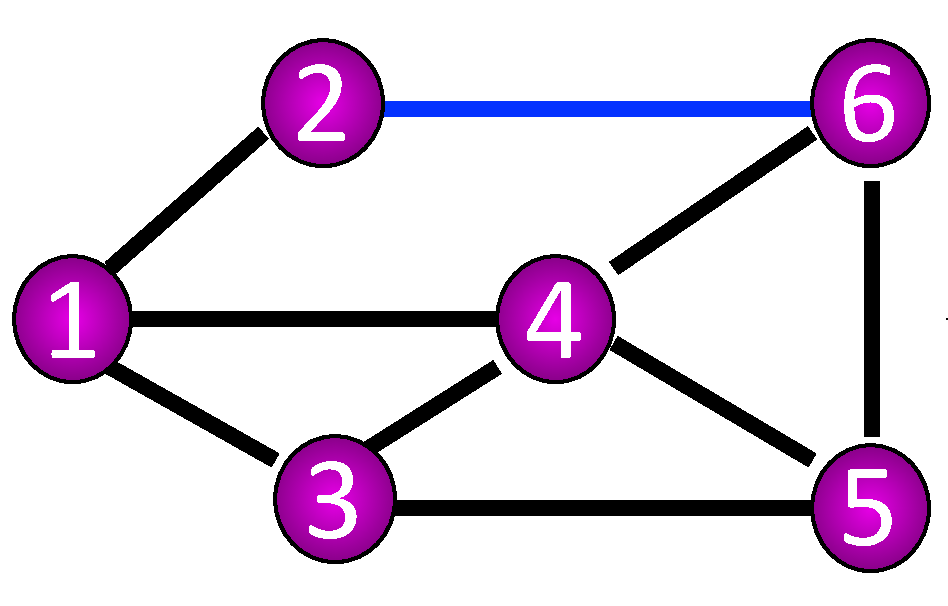
\includegraphics[width=0.45\textwidth]{graph.pdf}
		\end{figure}
		}
	\item Modeling real-world systems by graphs
	\footnotesize
	\begin{table}
		\centering
		%\caption[Caption for LOF]{Some classic real networks.\protect\footnotemark}
		%\caption{Some classic real networks.}
		\begin{tabular}{c|c|c}
			\hline
			\rowcolor{Gray}
			Real-world networks & Vertices & Edges \\
			\hline
			Social networks & People & Friendship/Interactions \\
			\hline
			The World Wide Web & Web pages & Web links \\
			\hline
			Power grid & Stations & Transmission lines \\
			\hline
		\end{tabular}
  \end{table}
  \end{itemize}
  \normalsize
}

\frame{
	\frametitle{Centrality in Networks}
	Indicators of \textbf{centrality} identify the most important vertices/edges, e.g.
	\begin{itemize}
		%\item Centrality is often used for detecting
		%	\begin{itemize}
				\item Identify influential persons in a social network
					\begin{itemize}
						\item Independent cascade model: measuring the importance of a person by its ability in information
							spreading
					\end{itemize}
				%\item How well used a road is in a transportation network
				\item Identify important web pages
					\begin{itemize}
						\item Google's PageRank algorithm: identifying important web pages by stationary distributions of random walks
					\end{itemize}
				\item Identify important transmission lines in a power grid
					\begin{itemize}
						\item Northeast blackout of 2003: failure of a few transmission lines in Cleveland causing
							a widespread power outage in North America
					\end{itemize}
		%	\end{itemize}
	\end{itemize}
}

\frame{
	\frametitle{Common Used Edge Centrality Measures}
	\begin{itemize}
		\item Comparing to vertex centrality, edge centrality measures are much less, due to computational challenge
		%\item Common used edge centrality for an edge \small $e \in E$ \normalsize
			\footnotesize
			\begin{table}
				\centering
				%\caption[Caption for LOF]{Some classic real networks.\protect\footnotemark}
				%\caption{Some classic real networks.}
				\begin{tabular}{c|c}
					\hline
					\rowcolor{Gray}
					Edge centrality name & Definition for an edge \scriptsize $e\in E$ \footnotesize \\
					\hline
					Betweenness \scriptsize $\mathcal{B}(e)$ \footnotesize &
						Fraction of shortest paths passing through \scriptsize $e$ \footnotesize \\
					\hline
					Spanning edge centrality \scriptsize $\mathcal{S}(e)$ \footnotesize &
						Fraction of spanning trees containing \scriptsize $e$ \footnotesize \\
					\hline
					Current-flow centrality \scriptsize $\mathcal{F}(e)$ \footnotesize &
						Average current flow passing through \scriptsize $e$ \footnotesize \\
					\hline
				\end{tabular}
		  \end{table}
		  \normalsize
		  
		  \item Weakness
		  	\begin{itemize}
		  		\item Betweenness: only considering shortest paths, ignoring even slightly longer paths
		  		\item Spanning edge centrality: lacking structure information
		  			\begin{itemize}
		  				\item A path and a star are both trees, while their structures differ
		  			\end{itemize}
				\item Current-flow centrality: hard to compute
		  	\end{itemize}

			%\begin{itemize}
			%	\item Betweenness \[\mathcal{B}(e) \defeq \text{fraction of shortest path passing through} e\]
			%	\item Spanning edge centrality $\mathcal{S}(e) \defeq $
			%\end{itemize}
	\end{itemize}
}

\frame{
	\frametitle{Effective Resistances}
	{
	\vspace{-10pt}
	\begin{wrapfigure}{L}{0.4\textwidth}
		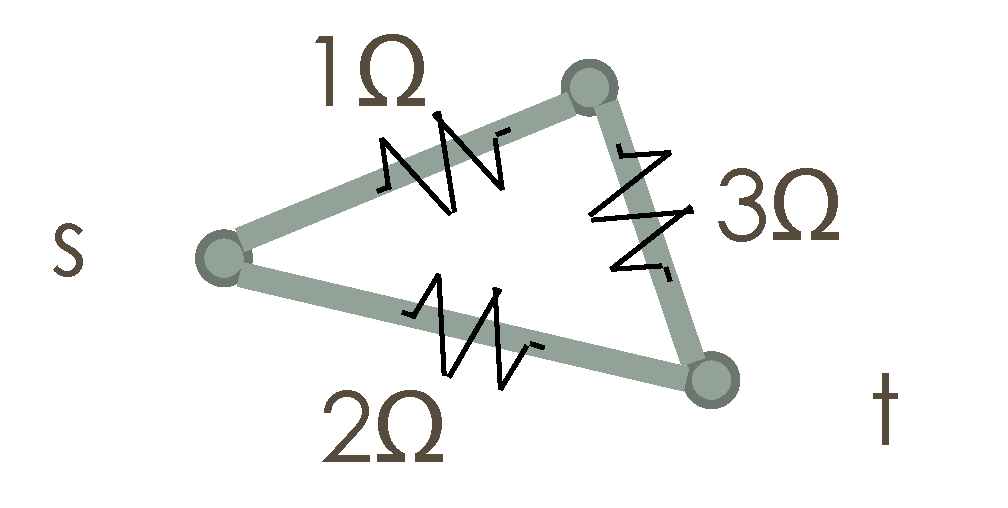
\includegraphics[width=0.4\textwidth]{resistances}
	\end{wrapfigure}
	\quad \\[1pt]
	\small
	\[ \er(s,t) = \frac{1}{\frac{1}{2} + \frac{1}{4}} = \frac{4}{3}\ \Omega \]
	\normalsize
	\quad \\[5pt]
	}
	\quad \\[2.5pt]
	\begin{itemize}
		\item The \textbf{effective resistance} \small$\er(s,t)$ \normalsize between \small$s,t$\, \normalsize is the \textit{electric resistance} between them in the whole electric network%. By Ohm's Law,
			%\small
			%\[
			%	\hspace{-10pt} \er(s,t) = \frac{\vv(s) - \vv(t)}{\ii(s,t)}
			%\]
			%\normalsize
		\item Connection to commute times in random walks
			\begin{itemize}
				\item \small The commute time \footnotesize$\kappa(s,t)$\small\ between
					\footnotesize$s,t$\,\small\ is the expected time of a random walk to go from
					\footnotesize$s \to t \to s$\small, and it is known that
					\vspace{-12pt}
					\footnotesize
					\[
						\kappa(s,t) = \mathrm{vol}(G) \er(s,t),
						\vspace{-16pt}
					\]
					\small
					where \footnotesize$\mathrm{vol}(G)$\small\ is the sum of degrees over all vertices
				\item Thus, \footnotesize$\er(s,t)$\small\ takes into account all paths between \footnotesize$s,t$
			\end{itemize}
	\end{itemize}
}

\frame{
	\frametitle{Kirchhoff Index}
	\begin{itemize}
		\item The \textbf{Kirchhoff index} \small$\mathcal{K}(G)$\normalsize\ of a graph \small$G$\normalsize\ 
			is defined as the sum of effective resistances over all vertex pairs, i.e.
			\small
			\vspace{-5pt}
			\[
				\mathcal{K}(G) = \sum\limits_{u,v} \er(u,v)
				\vspace{-5pt}
			\]
			\normalsize
		\item Kirchhoff index takes into account all paths in the graph
		\item Kirchhoff index measures the overall connectivity of the graph
		\item Kirchhoff index has applications to measuring
			\begin{itemize}
				\item The mean cost of search in a complex network
				\item Robustness of first-order consensus algorithm in noisy networks
				\item The global utility of social recommender systems
			\end{itemize}
	\end{itemize}
}

\frame{
	\frametitle{Kirchhoff Centrality}
	\begin{itemize}
		\item Rayleigh's Monotonicity Law
			\begin{itemize}
				\item \footnotesize$\mathcal{K}(G)$\small\ increases when edge conductance is decreased
					%(i.e. edge resistance increased)
				\item Thus, edge deactivation makes the graph less connected
			\end{itemize}
		\item An edge \small$e$\normalsize 's importance is reflected in the increase of Kirchhoff index when $e$ is deactivated
			\begin{itemize}
				\item Resembling the power grid case
			\end{itemize}
		\item \small$G\bsk e$\,\normalsize\ denotes multiplying conductance of \,\small$e$\,\normalsize\ by
			\small$\theta\in (0, 1/2]$\normalsize
			\footnotesize
			\begin{table}
				\centering
				%\caption[Caption for LOF]{Some classic real networks.\protect\footnotemark}
				%\caption{Some classic real networks.}
				\begin{tabular}{b|c}
					\hline
					\scriptsize$\theta$\footnotesize-Kirchhoff edge centrality \scriptsize$\mathcal{C}_\theta(e)$
					&
						\scriptsize$\mathcal{C}_\theta(e) \defeq \mathcal{K}(G\bsk e)$ \\
					\hline
					\scriptsize$\theta$\footnotesize-Kirchhoff edge centrality \scriptsize$\mathcal{C}_\theta^\Delta(e)$
					&
						\scriptsize$\mathcal{C}_\theta^\Delta(e) \defeq \mathcal{K}(G\bsk e) - \mathcal{K}(G)$ \\
					\hline
					\scriptsize$\theta$\footnotesize-Kirchhoff vertex centrality \scriptsize$\mathcal{C}_\theta^\Delta(v)$
					&
						\scriptsize$\mathcal{C}_\theta^\Delta(v) \defeq \mathcal{K}\kh{G\bsk N(v)} - \mathcal{K}\kh{G}$ \\
					\hline
				\end{tabular}
		  \end{table}
		  \normalsize
	\end{itemize}
}

\frame<0 | handout:0>{
	\frametitle{Comparison With Other Measures}
	\framesubtitle{Examples}
	{
	\vspace{-10pt}
	\begin{wrapfigure}{L}{0.4\textwidth}
		\hspace{10pt}
		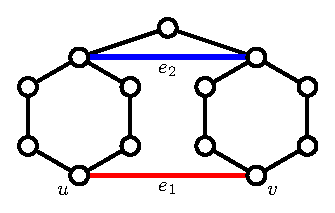
\includegraphics[width=0.4\textwidth]{s_1.eps}
	\end{wrapfigure}
	\quad \\[1pt]
	\small
	\[
		x
	\]
	\normalsize
	\quad \\[5pt]
	}
	\quad \\[20pt]
	{
	%\vspace{-10pt}
	\begin{wrapfigure}{L}{0.6\textwidth}
		\hspace{-20pt}
		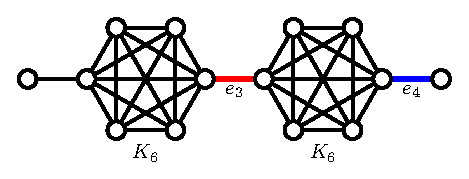
\includegraphics[width=0.6\textwidth]{r_1.eps}
	\end{wrapfigure}
	\quad \\[1pt]
	\small
	\[
		x
	\]
	\normalsize
	\quad \\[5pt]
	}
}

\frame{
	\frametitle{Comparison With Other Measures}
	\framesubtitle{Examples}
	\begin{figure}
		\vspace{10pt}
		\makebox[\linewidth][c]{
		\begin{subfigure}[H]{0.4\textwidth}
			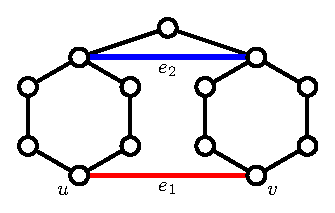
\includegraphics[width=1\textwidth]{s_1.eps}
			%\caption{The first 3 eigenvalues of $B$}
		\end{subfigure}
		\quad\quad\,
		\begin{subfigure}[H]{0.6\textwidth}
			\vspace{10pt}
			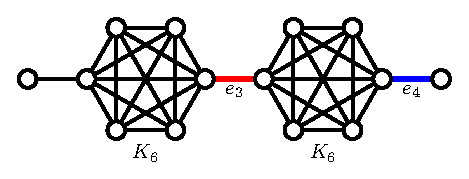
\includegraphics[width=1\textwidth]{r_1.eps}
		\end{subfigure}
		}
		\vspace{2pt}
		%\caption{The accuracy of spectral clustering based on different matrices}
	\end{figure}
	\begin{itemize}
		\item \small Betweenness cannot distinguish between \footnotesize$e_1$\small\ and \footnotesize$e_2$\small
				\footnotesize
				\vspace{-10pt}
				\begin{align*}
					&\mathcal{B}(e_1) = \mathcal{B}(e_2) = 18 \\[0.001cm]
					&\mathcal{C}_{0.1}(e_1) = 132.65,\ \mathcal{C}_{0.1}(e_2) = 112.34
				\end{align*}
				\vspace{-25pt}
		\item \small Spanning edge centrality cannot distinguish between \footnotesize$e_3$\small\ and \footnotesize$e_4$\small
				\footnotesize
				\vspace{-10pt}
				\begin{align*}
					&\mathcal{S}(e_3) = \mathcal{S}(e_4) = 1 \\[0.001cm]
					&\mathcal{C}_{0.1}(e_3) = 467.33,\ \mathcal{C}_{0.1}(e_4) = 197.33
				\end{align*}
				%\vspace{-15pt}
	\end{itemize}
}

\frame{
	\frametitle{Comparison With Other Measures}
	\framesubtitle{Experiments}
	\begin{figure}
		%\vspace{10pt}
		\makebox[\linewidth][c]{
			%\begin{table}
	\centering
	\hspace{-15pt}
	\footnotesize
	\begin{tabular}{|c|c|c|}
		\hline
		\rowcolor{Gray}
		Network name & $\sizeof{V}$ & $\sizeof{E}$ \\
		\hline
		Karate & 34 & 78 \\
		\hline
		Lesmis & 77 & 254 \\
		\hline
		Adjnoun & 112 & 425 \\
		\hline
		Dolphins & 62 & 159 \\
		\hline
		Celegansneural & 297 & 2148 \\
		\hline
	\end{tabular}
	%\end{table}
	\quad
	\begin{subfigure}[H]{0.6\textwidth}
		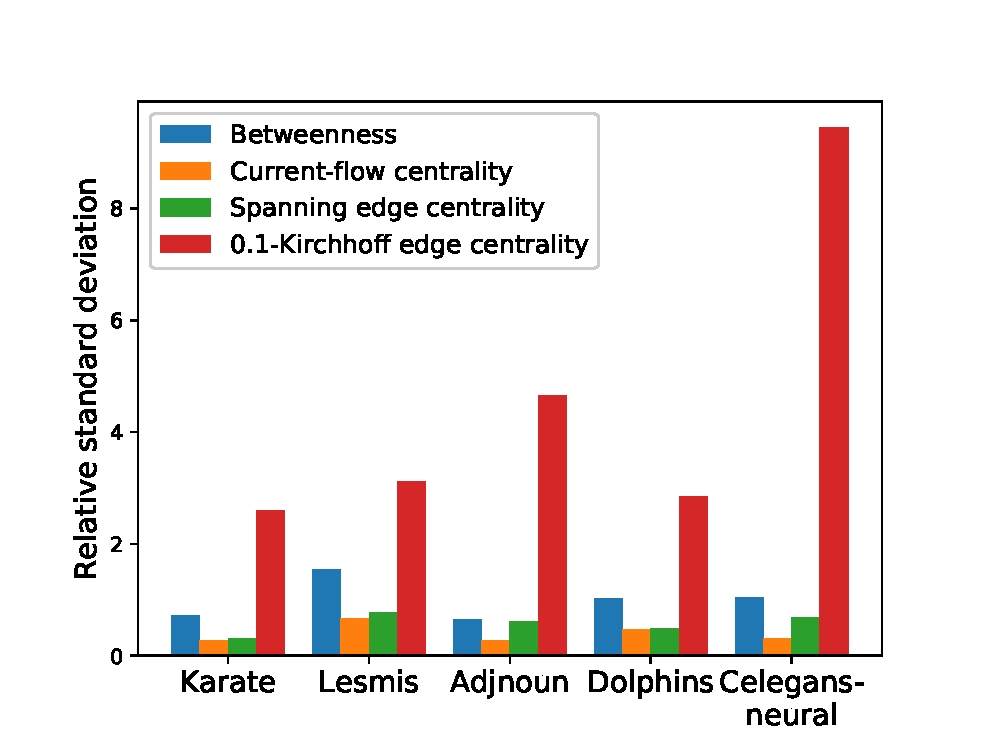
\includegraphics[width=1.2\textwidth]{deviation.eps}
	\end{subfigure}
	}
	\vspace{5pt}
	\end{figure}
%	\small
	\[
		\text{Relative standard deviation} \,\,\defeq \quad \frac{\text{Standard deviation}}{\text{Average}}
	\]
	%}
	%{
	%\begin{wrapfigure}{L}{0.55\textwidth}
%		\hspace{-30pt}
%		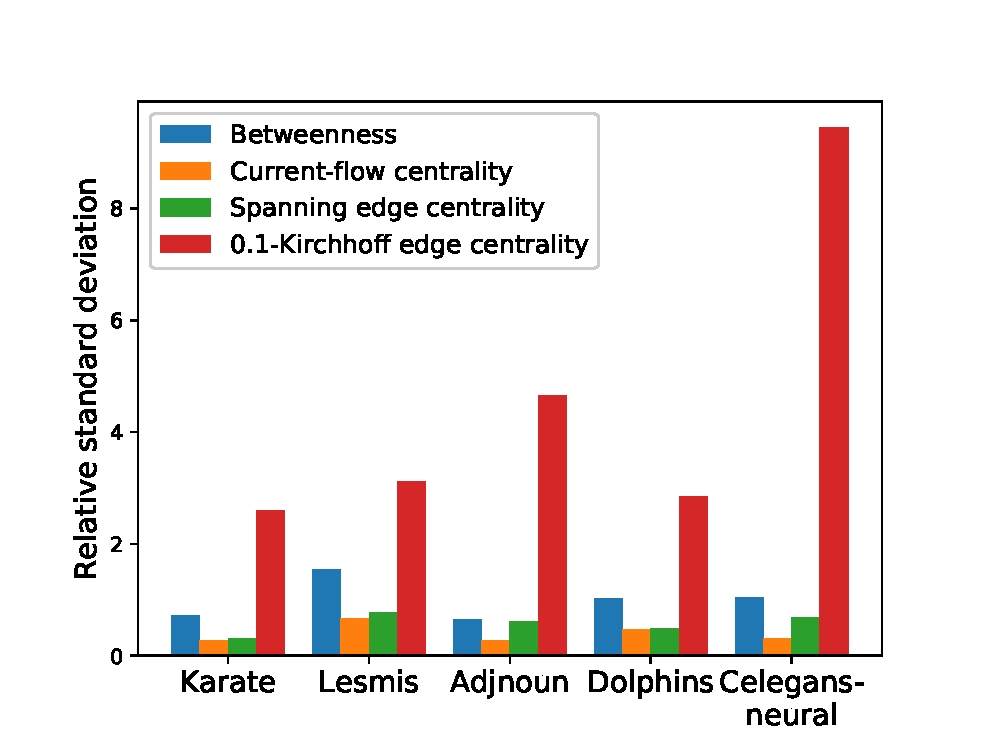
\includegraphics[width=0.7\textwidth]{deviation.eps}
%		\hspace{-30pt}
%	\end{wrapfigure}
%	\quad \\[20pt]
%	\small 
%	\begin{align*}
%		&\text{relative standard deviation}\\
%			\defeq \quad &\frac{\text{standard deviation}}{\text{average}}
%	\end{align*}
%%	\quad \\[5pt]
	%}
}

\section{Nearly Linear Time Algorithms}

\frame{\frametitle{Outline} \tableofcontents[currentsection]}
			
\subsection{(Approximate) Schur complements and Cholesky factorization}
%\subsection{Approximate Gaussian elimination for Laplacians}
\subsection{Johnson-Lindenstrauss lemma and Hutchinson's trace estimation}
\subsection{Offline divide and conquer}
\subsection{Sherman-Morrison and Woodbury formulas}

\frame{
	\frametitle{Graph Laplacians}	
	\insfig[0.45]{lapl}
	\scriptsize
	%\begin{table}
	%	\centering
	%	\begin{tabular}{c|c}
	%		\hline
	\vspace{-12pt}
			\begin{align*}
			\LL &= \DD - \AA = 
			\begin{pmatrix}
				3 & 0 & 0 \\
				0 & 4 & 0 \\
				0 & 0 & 5
			\end{pmatrix}
			-
			\begin{pmatrix}
				0 & 1 & 2 \\
				1 & 0 & 3 \\
				2 & 3 & 0
			\end{pmatrix}\\[5pt]
			&= \sum\limits_{e\in E}w(e) \bb_{e}\bb_{e}^T =
			\begin{pmatrix}
				1 & -1 & 0 \\
				-1 & 1 & 0 \\
				0 & 0 & 0
			\end{pmatrix}
			+
			\begin{pmatrix}
				2 & 0 & -2 \\
				0 & 0 & 0 \\
				-2 & 0 & 2
			\end{pmatrix}
			+
			\begin{pmatrix}
				0 & 0 & 0 \\
				0 & 3 & -3 \\
				0 & -3 & 3
			\end{pmatrix}
			\end{align*}% \\
			%\hline
		%\end{tabular}
	%\end{table}
	\footnotesize
	where\, \scriptsize$\bb_{e} = \bb_{u,v} = \ee_u - \ee_v$\,\footnotesize\ 
	for an edge \scriptsize$e = (u,v) \in E$
}

\frame{
	\frametitle{Turning Kirchhoff Index into Trace of Pseudoinverse}
	\quad\\[8pt]
	\begin{itemize}
		\item
		\footnotesize $\LL = \sum\nolimits_{i=1}^{n} \lambda_i \vv_i \vv_i^T$,\ \,
		\footnotesize $\LL^\dag = \sum\nolimits_{i=2}^{n} \frac{1}{\lambda_i} \vv_i \vv_i^T$\small\ \, where\\[3pt]
			\begin{itemize}
				\item \scriptsize$0 = \lambda_1 \leq \lambda_2 \leq\ldots\leq \lambda_n$\,\footnotesize\ 
					are eigenvalues of \scriptsize$\LL$
				\item \scriptsize$\one = \vv_1, \vv_2, \ldots, \vv_n$\,\footnotesize\ are the orthonormal eigenvectors
			\end{itemize}\vspace{2pt}
		\item \footnotesize $\er(u,v) = \bb_{u,v}^T \LL^\dag \bb_{u,v}$\vspace{7pt}
		\item \footnotesize $\mathcal{K}(G) = n\,\trace{\LL^\dag}$%\vspace{5pt}
			\scriptsize
			\begin{align*}
				\mathcal{K}(G) &= \sum\limits_{u,v} \er(u,v) = \sum\limits_{u,v} \bb_{u,v}^T \LL^\dag \bb_{u,v} \\
				&= \sum\limits_{u,v} \trace{\LL^\dag \bb_{u,v} \bb_{u,v}^T}
				= \trace{\LL^\dag \sum\limits_{u,v} \bb_{u,v} \bb_{u,v}^T} \\[5pt]
				&= \trace{\LL^\dag \LL_{K_n}} = \trace{\LL^\dag \kh{n\II - \one\one^T}} = n\trace{\LL^\dag}
			\end{align*}
	\end{itemize}
}

\frame{
	\frametitle{Gaussian Elimination and LU Factorization}
}

\frame{
	\frametitle{Cholesky Factorization for Laplacians}
}

\frame{
	\frametitle{Clique Structure of Schur Complements}
}

\frame{
	\frametitle{Multiplicative Approximation}
}

\frame{
	\frametitle{Sparsification of Schur Complements}
}

\frame{
	\frametitle{Solving \large$\LL\xx = \bb$}
}

\frame{
	\frametitle{Estimating Trace of an Implicit Matrix}
}

\frame{
	\frametitle{Estimating Trace by JL}
}

\frame{
	\frametitle{Approximating \large$\trace{\LL^\dag}$\Large\ in Nearly Linear Time}
}

\frame{
	\frametitle{Offline Div-conquer (离线分治): OI version}
	\vspace{-5pt}
	\begin{figure}
		\makebox[\linewidth][c]{
		\begin{subfigure}[H]{0.58\textwidth}
			
\includegraphics[width=1\textwidth]{cdq2}
			\label{exp1}	
			\caption{Dynamic programming by div-conquer}
		\end{subfigure}
		\begin{subfigure}[H]{0.5\textwidth}
			\vspace{24pt}
			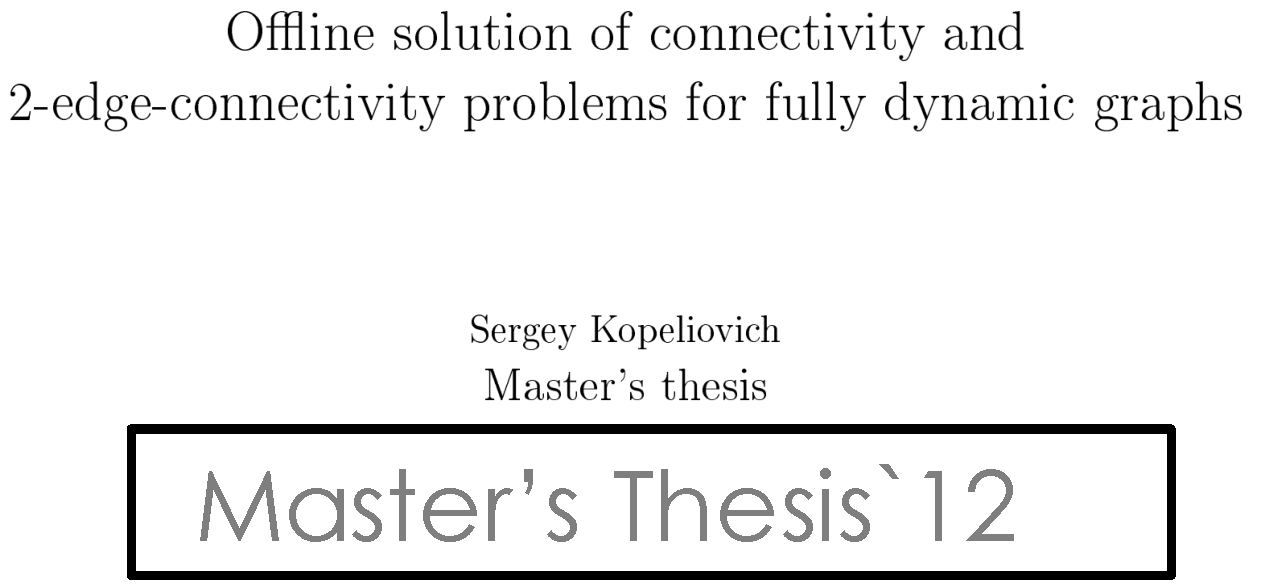
\includegraphics[width=1\textwidth]{master12}
			\label{exp2}
			\caption{Dynamic connectivity by div-conquer}
		\end{subfigure}
		}
		\\[-2pt]
		\makebox[\linewidth][c]{
		\begin{subfigure}[H]{0.58\textwidth}
			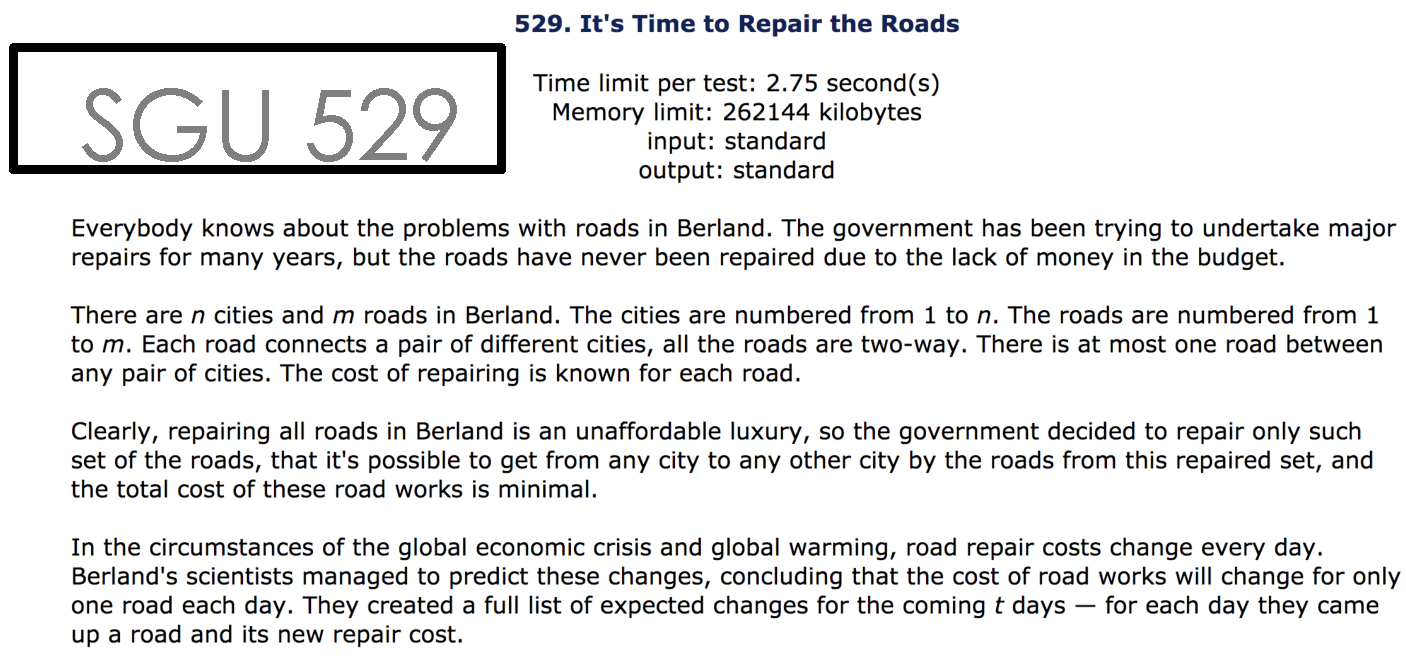
\includegraphics[width=1\textwidth]{sgu_short}
%			\vspace{-25pt}
			\label{exp1}
			\caption{Maintaining MST under updates in \scriptsize$\tilde{O}(m)$}
		\end{subfigure}
		\begin{subfigure}[H]{0.58\textwidth}
			\vspace{14pt}
			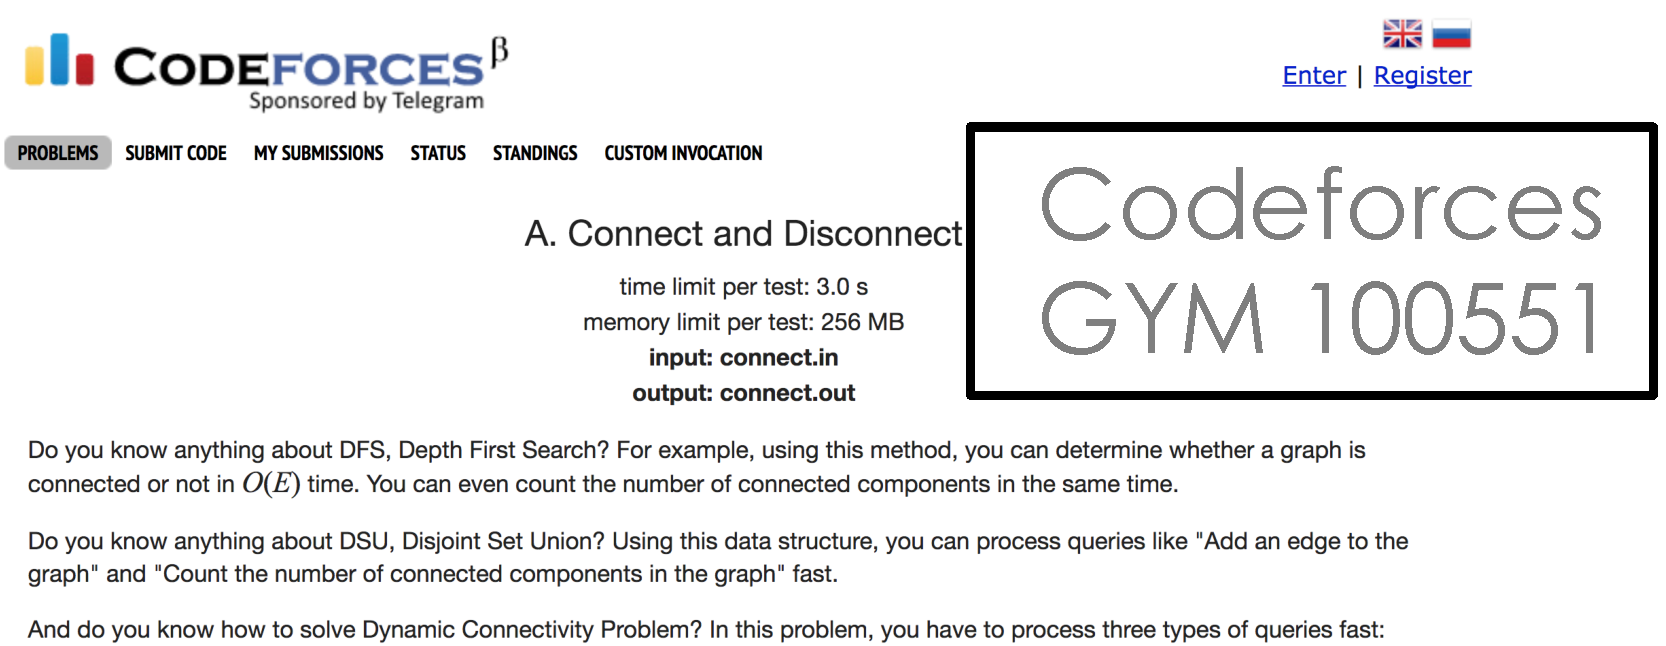
\includegraphics[width=1\textwidth]{cf100551}
			%\vspace{0.1pt}
			\label{exp2}
			\caption{Maintaining \#CC under updates in \scriptsize$\tilde{O}(m)$}
		\end{subfigure}
		}
		%\caption{The spectrum of $A$ (left) and $B$ (right)}
	\end{figure}
}

\frame{
	\frametitle{Algorithms That Use Div-conquer}
}

%%%%%%%%%%%%%%%%%%%%%%%%%%%%%%%%%%%%%%%%%%%%%%%%%%%%%%%%%%%%%%%%%%%%%%%%%%%%%%%%%%%%%%%%%%%%%%%%%%%%%

\frame{
	\frametitle{Clustering by the Laplacian $L = D - A$\footnote[frame]{Ulrike Luxburg (2007). A tutorial on spectral clustering. Statistics and Computing,
17(4):395-416.}}
	%\begin{block}{Unnormalized spectral clustering}
	Input: Adjacency matrix $A \in \mathbb{R}^{n\times n}$, number of clusters $q$
	
	\begin{itemize}
		\item $q = 2$
			\begin{itemize}
				\item Cluster by the signs of the 2nd eigenvector of $L$
			\end{itemize}
		\item $q > 2$
			\begin{itemize}
				\item Let $u_1, \cdots, u_q$ be the first $q$ eigenvectors of $L$ %\vspace{5pt}
				\item Let $ U = (u_1, \cdots, u_q) \in \mathbb{R}^{n\times q}$ %\vspace{5pt}
				\item Let $ 
				\begin{pmatrix}
					y_1 \\ \vdots \\ y_n
				\end{pmatrix}
				= U
				$
				%\vspace{5pt}
				\item Cluster the points $y_1, \cdots, y_n \in \mathbb{R}^q$ with $k$-means
			\end{itemize}
	\end{itemize}
	%\end{block}
}
\note{
	\begin{itemize}
		\item 最早提出的谱聚类方法: 用\ Laplacian\ 聚类
	\end{itemize}
}

\frame{
	\frametitle{Clustering by the Adjacency Matrix $A$\footnote[frame]{Avrim Blum, John Hopcroft, and Ravindran Kannan (2016). Foundations of Data Science (pp. 275-281).}}
	\insfig{Spectral_Clustering}
}
\note{
	\begin{itemize}
		\item 邻接矩阵\ 而不是\ Laplacian
	\end{itemize}
}

\frame{
	\frametitle{Spectral Clustering in Sparse Networks}
	\begin{itemize}
		\item Clustering based on $A$ fails to detect communities
		\vspace{5pt}
		\item Locally tree-like structure
		\vspace{5pt}
		\item Leading eigenvalues of $A$ are dictated by the vertices of highest degree\footnote[frame]{Michael Krivelevich and Benny Sudakov (2003). The largest eigenvalue of sparse
random graphs. Combinatorics, Probability and Computing, 12(01):61-72.}
		\vspace{5pt}
		\item Corresponding eigenvectors are localized around these vertices\footnotemark[\value{footnote}]
	\end{itemize}
}
\note{
	\begin{itemize}
		\item 稀疏图:Laplacian\ 或\ 邻接矩阵\ 聚类效果不好
		\item 原因:对于稀疏图:
			\begin{itemize}
				\item 最大的一些特征值\ 受到\ 度数比较大的点
				\item 对应的特征向量\ 聚集在\ 度数比较大的点上
			\end{itemize}
		\item 更进一步\ 的\ 原因
			\begin{itemize}
				\item locally tree-like structure
				\item 树上的\ Eigenvalues and Eigenvectors\ 受到\ 度数大的点的影响\ 非常大
			\end{itemize}
		\item Star 图\ 的例子
	\end{itemize}
}

\frame{
	\frametitle{Clustering by the Non-Backtracking Matrix\footnote[frame]{Florent Krzakala, Cristopher Moore, et al (2013). Spectral redemption in clustering
sparse networks. Proceedings of the National Academy of Sciences, 110(52):20935–20940.}}
	\begin{itemize}
		\item The $2m\times 2m$ non-backtracking matrix $B$
		\[
		B_{(u \to v),(x \to y)} = \begin{cases} 
		1 & \mbox{if $v=x$ and $u \ne y$} \\
		0 & \mbox{otherwise} \, . 
		\end{cases}
		\]
		\item The spectrum of $B$ is not sensitive to high-degree vertices
		%\begin{itemize}
		%	\item A tree contributes zero eigenvalues to the spectrum
		%\end{itemize}
		\item Properties of $B$
			\begin{itemize}
				\item A tree contributes zero eigenvalues to the spectrum
				\item Unicyclic components yield eigenvalues either $1$ or $-1$
			\end{itemize}

	\end{itemize}
}


\frame{
	\frametitle{Stochastic Block Model}
	\vspace{-5pt}
	\begin{itemize}
		\item Stochastic block model
			\begin{itemize}
				\item $q$ groups of vertices with size $n/q$
				\item Each vertex $v$ has a group label $g_v \in \{1, \cdots, q\}$
				\item Adjacency matrix $A$ is generated according to the distribution \vspace{-7.5pt}
				\[
					\Pr[A_{u,v}=1] = \begin{cases}	
						\cin / n & g_u = g_v \\
						\cout / n & g_u \neq g_v 
					\end{cases},
					\mbox{where}\ \cin > \cout
				\]
			\end{itemize}
		\item \vspace{-5pt} Average degree $c = (\cin + \cout)/2$ \hspace{1pt} when $q = 2$
			%\begin{itemize}
			%	\item $L = D - A \approx c\id - A$
			%	\item Clustering by the second largest eigenvector of $A$
			%\end{itemize}
		\item $G$ becomes sparse when $n$ is large
			%\begin{itemize}
			%	\item Spectral clustering by $A$ fails
			%\end{itemize}
	\end{itemize}
}

\frame{
	\frametitle{Spectrum of $A$ and $B$}
%	\vspace{-5pt}
	\vspace{-5pt}
	\begin{figure}
		\makebox[\linewidth][c]{
		\begin{subfigure}[H]{0.45\textwidth}
			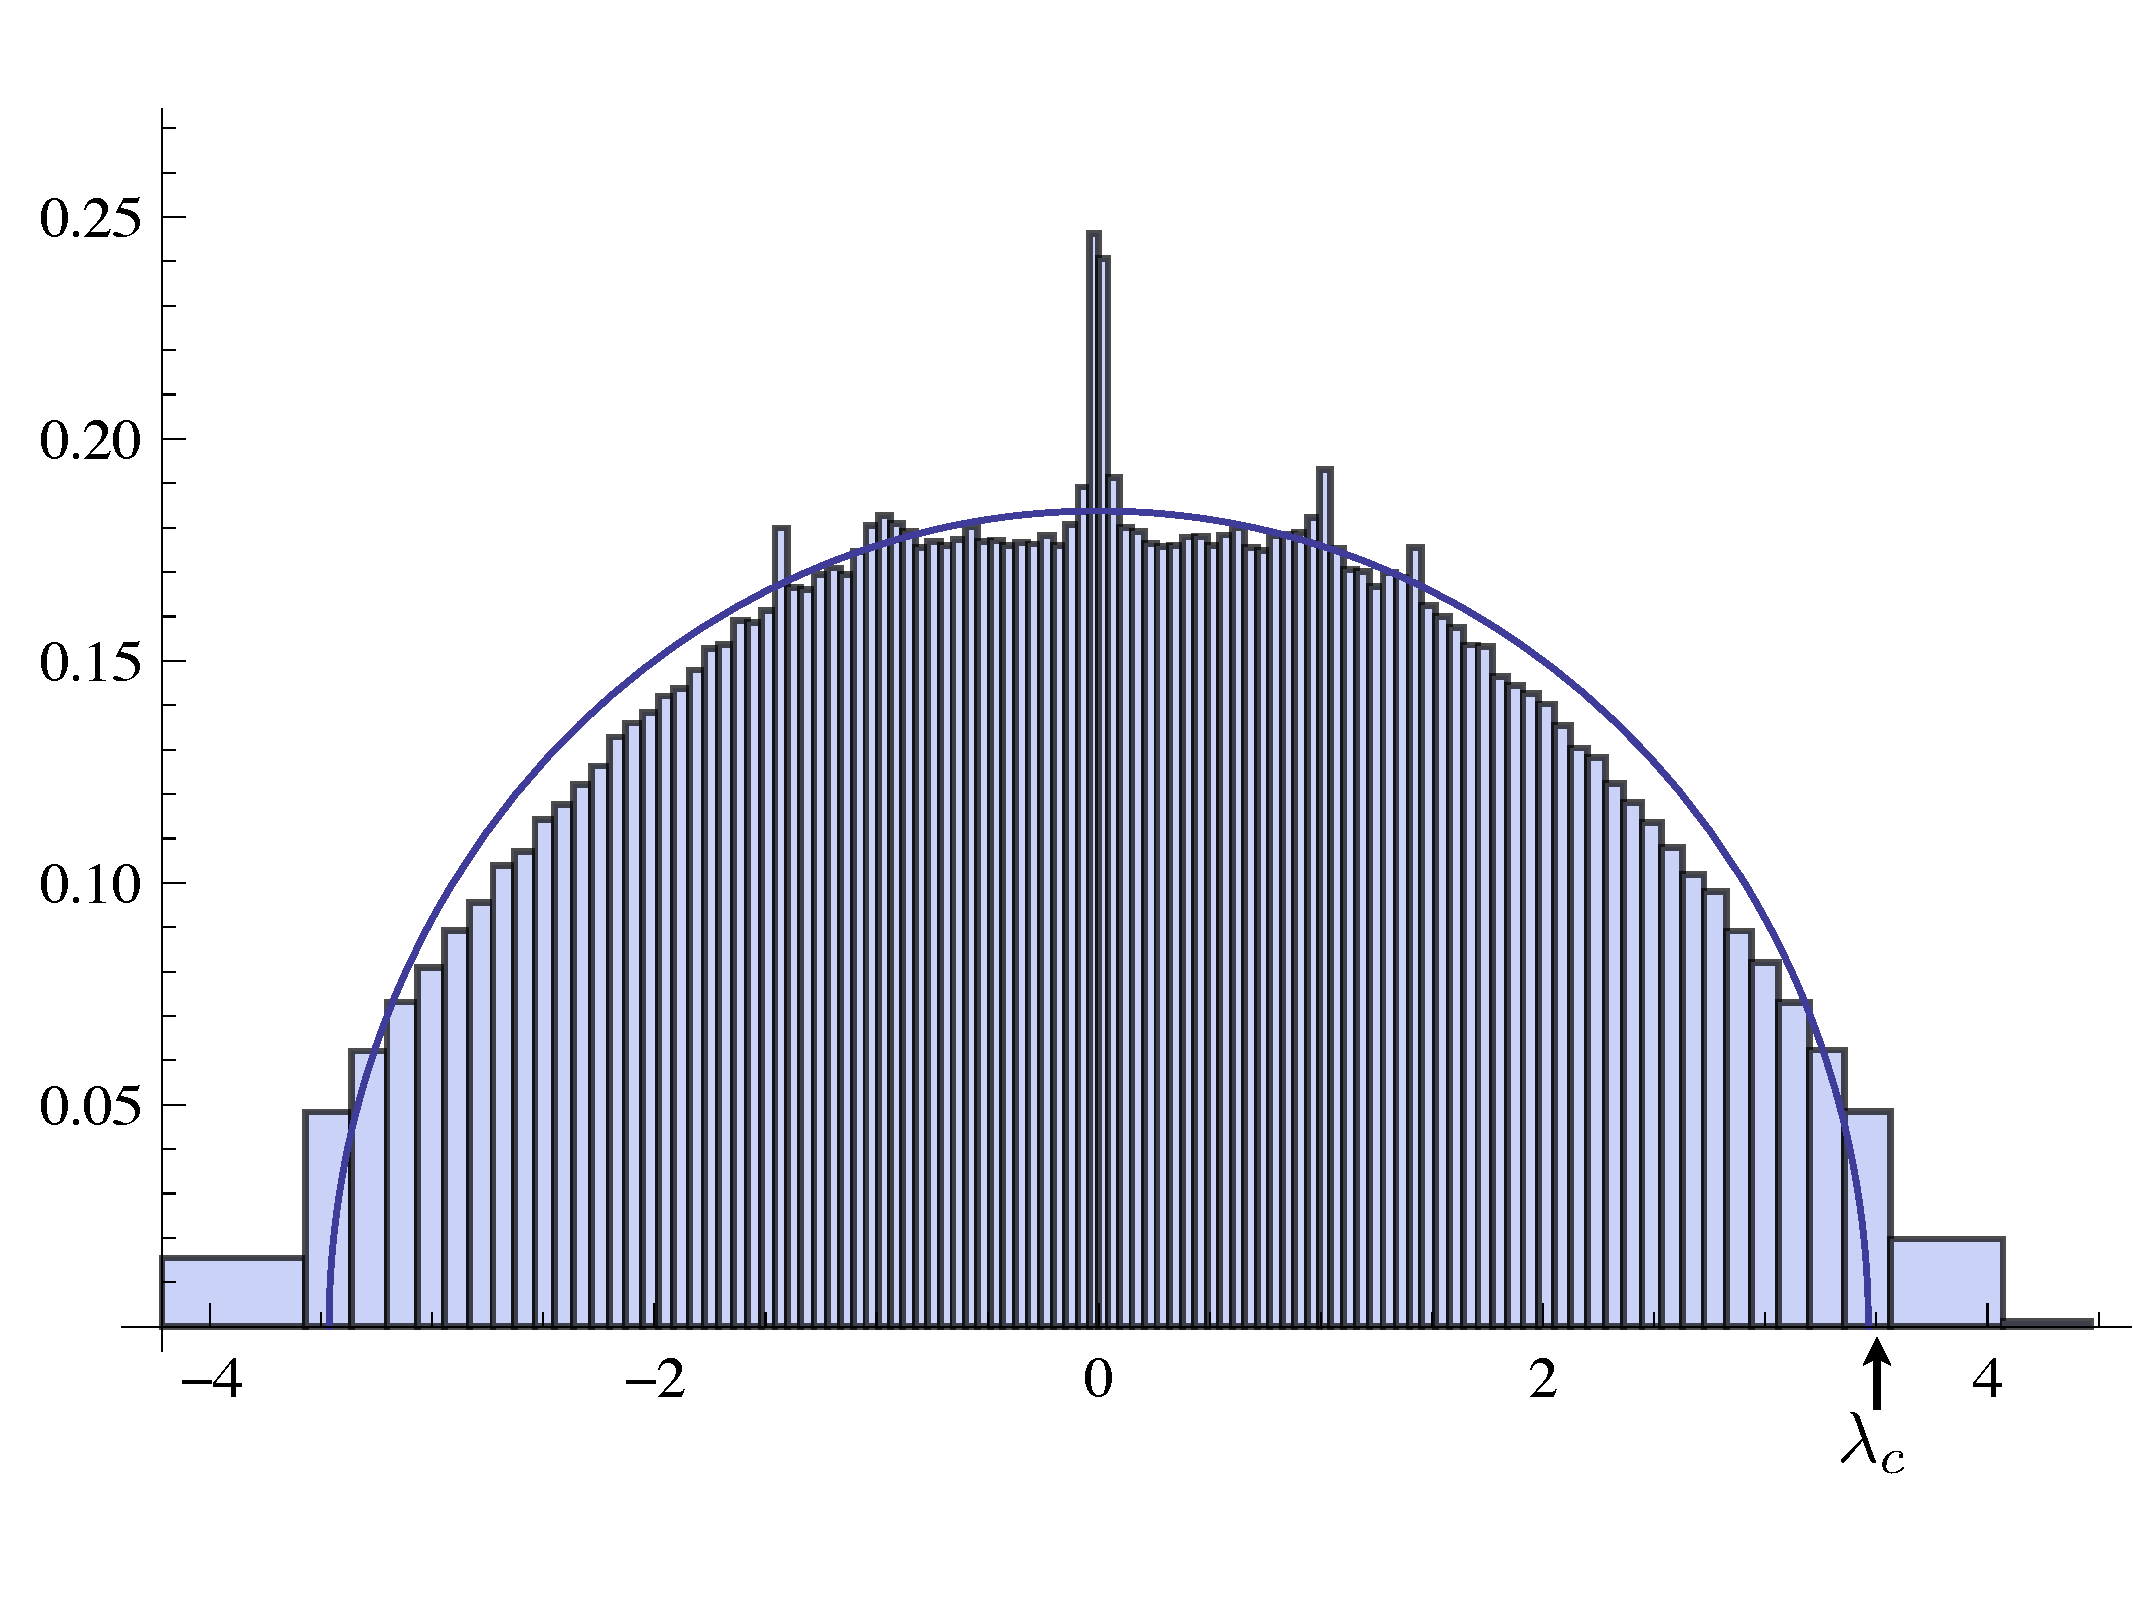
\includegraphics[width=1\textwidth]{EXP1}
			\label{exp1}
			\caption{The spectrum of $A$}
		\end{subfigure}
		\hspace{20pt}
		\begin{subfigure}[H]{0.45\textwidth}
			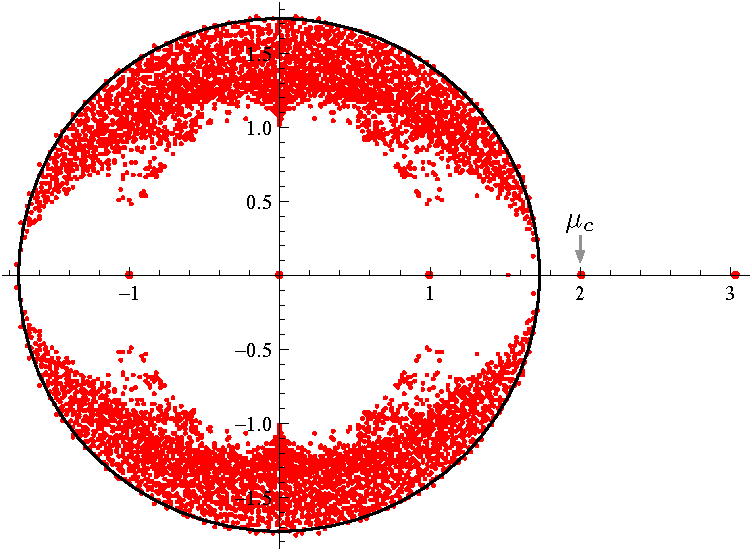
\includegraphics[width=1\textwidth]{EXP2}
			\label{exp2}
			\caption{The spectrum of $B$}
		\end{subfigure}
		}
		%\caption{The spectrum of $A$ (left) and $B$ (right)}
	\end{figure}
	\begin{itemize}
		\item $n = 4000$, $\cin = 5$, $\cout = 1$, $c = (\cin + \cout)/2 = 3$
		\item The radius of the bulk
			\begin{itemize}
				\item For $A$, $2\sqrt{c} = 3.46$
				\item For $B$, $\sqrt{c} = 1.73$
			\end{itemize}
	\end{itemize}
}
\note{
	\begin{itemize}
		\item SBM\ 的\ 参数
		\item 半圆\ 和\ 圆的半径
			\begin{itemize}
				\item 意义
				\item 取值
			\end{itemize}
		\item 第二大特征值\ $\lambda_c$\ 和\ $\mu_c$
	\end{itemize}
}

\frame{
	\frametitle{Experiments $n = 10^5$}	
	\begin{figure}
		\makebox[\linewidth][c]{
		\begin{subfigure}[H]{0.45\textwidth}
			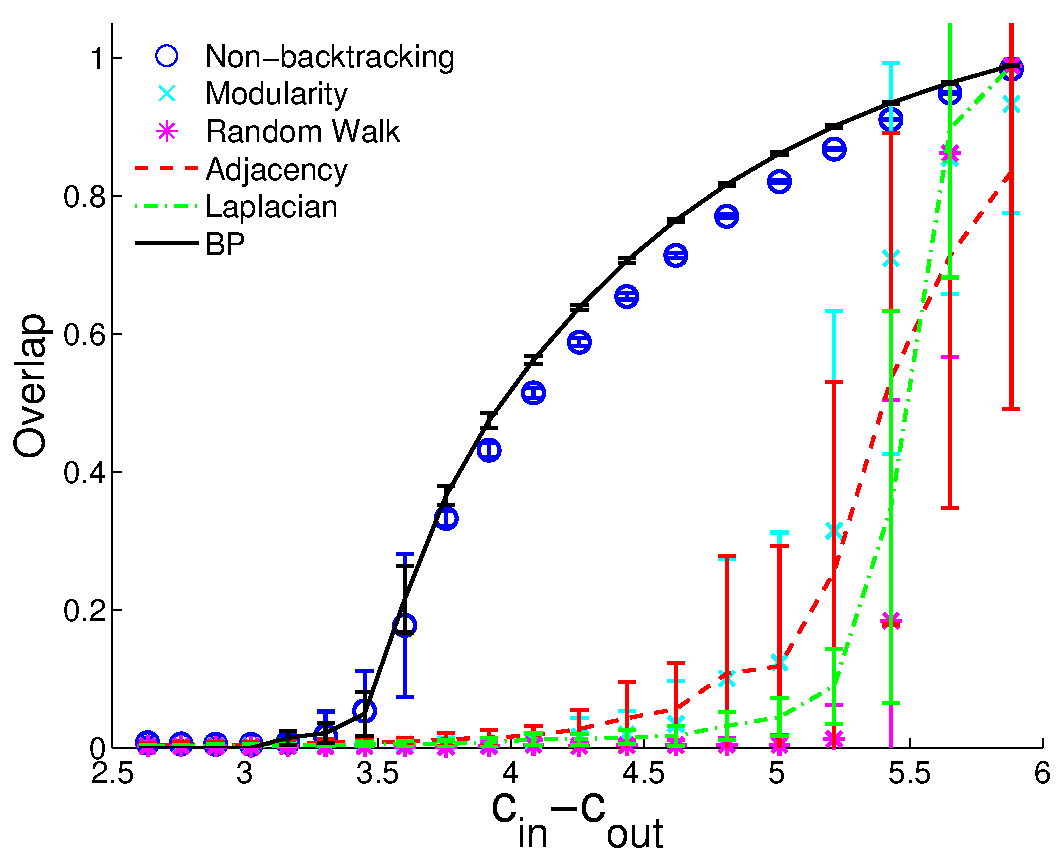
\includegraphics[width=1\textwidth]{EXP3}
			%\caption{The first 3 eigenvalues of $B$}
		\end{subfigure}
		\quad
		\begin{subfigure}[H]{0.45\textwidth}
			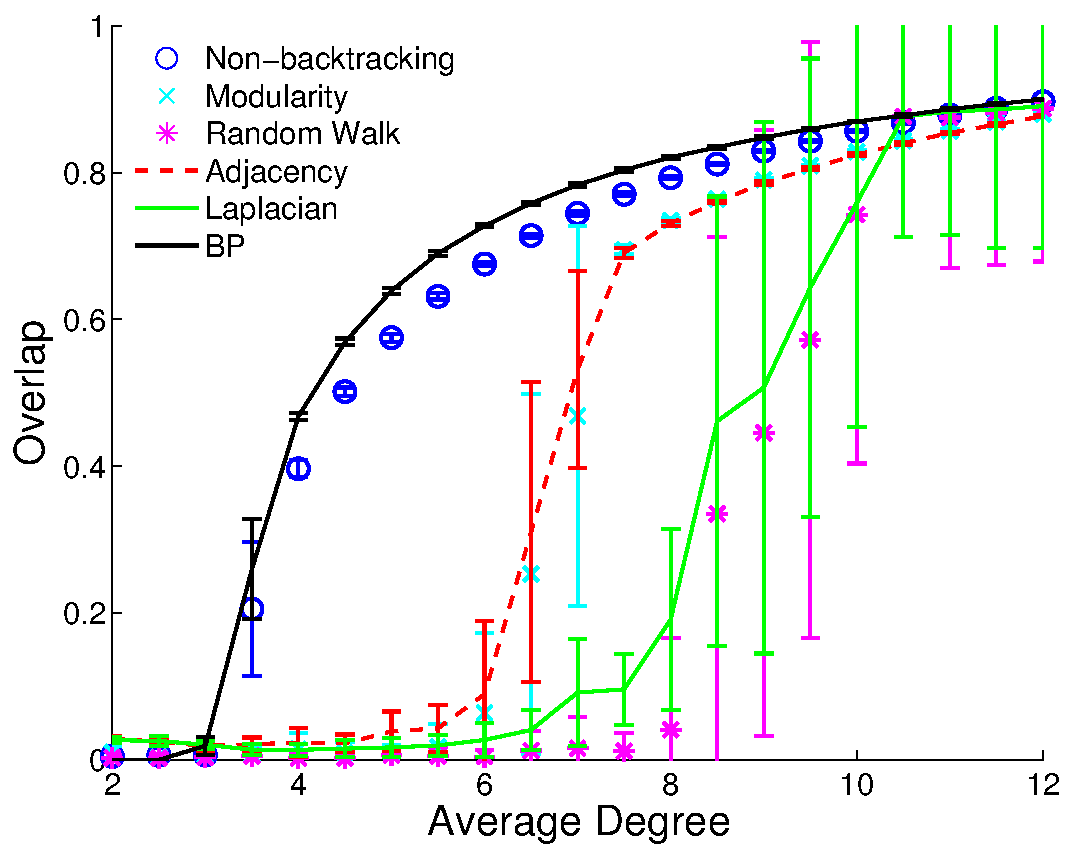
\includegraphics[width=1\textwidth]{EXP4}
		\end{subfigure}
		}
		%\caption{The accuracy of spectral clustering based on different matrices}
	\end{figure}
	\vspace{-5pt}
	\begin{itemize}
		%\item $n = 10^5$
			%\begin{itemize}
			%	\item On the left, set $c = 3$ and vary $\cin - \cout$
			%	\item On the right, set $\cout/\cin = 0.3$ and vary $c$
			%\end{itemize}
		\item $\mbox{Overlap} \triangleq
        \left( \frac{1}{n} \sum_u \delta_{g_u , \tilde{g}_u} -
          \frac{1}{q}\right) \Big{/} \left( 1 -  \frac{1}{q} \right)
$
		\vspace{5pt}
		\item Theoretical threshold\footnote[frame]{Elchanan Mossel, Joe Neeman, and Allan Sly (2012). Stochastic block models and
reconstruction. arXiv preprint, arXiv:1202.1499.} $\approx 3.46$
	\end{itemize}
}
\note{
	\begin{itemize}
		%\item 在\ SBM\ 生成的网络上\ 跑\ 不同的谱聚类方法
		\item 衡量标准:Overlap
		\item SBM\ 的\ 参数
			\begin{itemize}
				\item 左:$c = 3$,\ 增加\ $\cin - \cout$
				\item 右:$\cout / \cin = 0.3$, 增加\ $c$\
			\end{itemize}
		\item 理论阈值
	\end{itemize}
}

\frame{
	\frametitle{Detecting Number of Clusters}
	\begin{figure}
		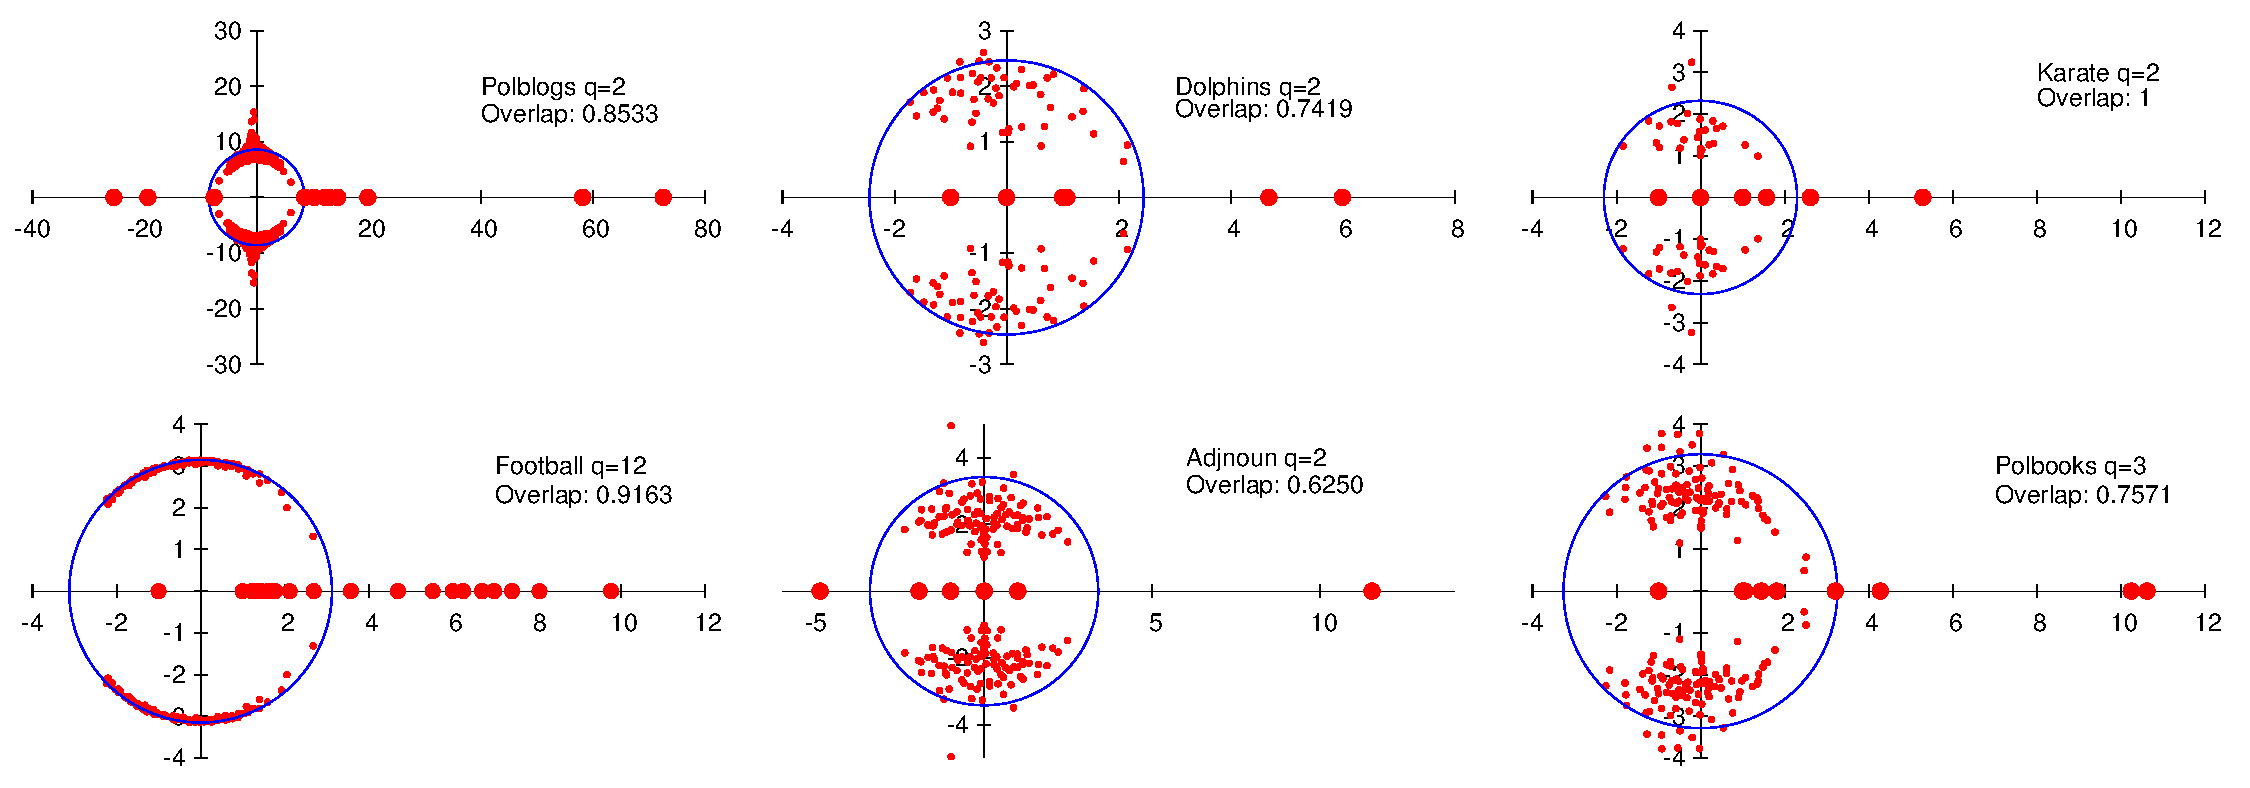
\includegraphics[width=1\textwidth]{DNOC}
		%\hspace*{8cm}
		\begin{itemize}
			\item Each circle's radius is $\sqrt{\rho(B)}$
			\item The number of real eigenvalues outside the circle indicates the number $q$ of clusters
		\end{itemize}
	\end{figure}
}
\note{
	\begin{itemize}
		\item 实际网络
		\item 检测社团个数
		\item 这一点\ Laplacian 或 Adjacency\ 都做不到
	\end{itemize}
}


\frame{
	\frametitle{Reducing the Computational Complexity}
	\vspace{-11.8pt}
	\begin{itemize}
		\item All eigenvalues $\lambda$ of $B$ not $\pm 1$ are the roots of the equation\footnote[frame]{Omer Angel, Joel Friedman, and Shlomo Hoory (2015). The non-backtracking spectrum of the universal cover of a graph. Trans. Amer. Math. Soc., 367(6):4287-4318.}
		\vspace{-10pt}
		\begin{equation} 
			\label{eq:ihara}
			\det[H(\lambda)] = \det \left[ \lambda^2 \id - \lambda A + (D-\id) \right] = 0 \,
		\end{equation}
		\item \vspace{-10pt} By the first companion linearization\footnote[frame]{Francoise Tisseur and Karl Meerbergen (2001). The quadratic eigenvalue problem. SIAM
Review, 43(2):235-286.}, roots of eq.~(\ref{eq:ihara}) are eigenvalues of \vspace{-10pt}
		\begin{equation}
			\label{eq:2nby2n}
			B' = \begin{pmatrix}
			0 & D-\id \\
			-\id & A
			\end{pmatrix}\quad \quad \quad \quad \nonumber
		\end{equation}
		\item \vspace{-2.5pt} Clustering by a $2n\times 2n$ matrix rather than a $2m\times 2m$ one
	\end{itemize}
}

\frame{
	\frametitle{The Bethe Hessian Matrix}
	\vspace{-9pt}
	\begin{itemize}
		\item All eigenvalues $\lambda$ of $B$ not $\pm 1$ are the roots of the equation
		\vspace{-10pt}
		\begin{equation} 
			\label{eq:ihara}
			\det[H(\lambda)] =  \det \left[ \lambda^2 \id - \lambda A + (D-\id) \right] = 0 \,
			\tag{1}
		\end{equation}
	\item The Bethe Hessian matrix $H(r)$
			\[
				\quad \ \ H(r):=r^2\id-rA+(D - \id) %\quad \quad  \quad \quad \quad
			\]
			\item $\forall$ real eigenvalue $\lambda$ of $B$, $H(\lambda)$ has a eigenvalue 0
			\begin{itemize}
				\item $H(\lambda\only<1-1>{\hspace{4.75pt}}\only<2-2>{_2})$'s null space \hspace{2pt} $\longleftrightarrow$ \hspace{2pt} $B$'s eigenvector corresponding to $\lambda\only<1-1>{\hspace{4.75pt}}\only<2-2>{_2}$
				\item Let $r_c = \sqrt{\rho(B)}$
				\item Eigenvectors of $H(r_c)$'s negative eigenvalues reveal clustering
			\end{itemize}
	\end{itemize}
}

\frame{
	\frametitle{Spectrum of $B$ and $H(r)$}
	\vspace{-20pt}
	\begin{wrapfigure}{L}{0.55\textwidth}
		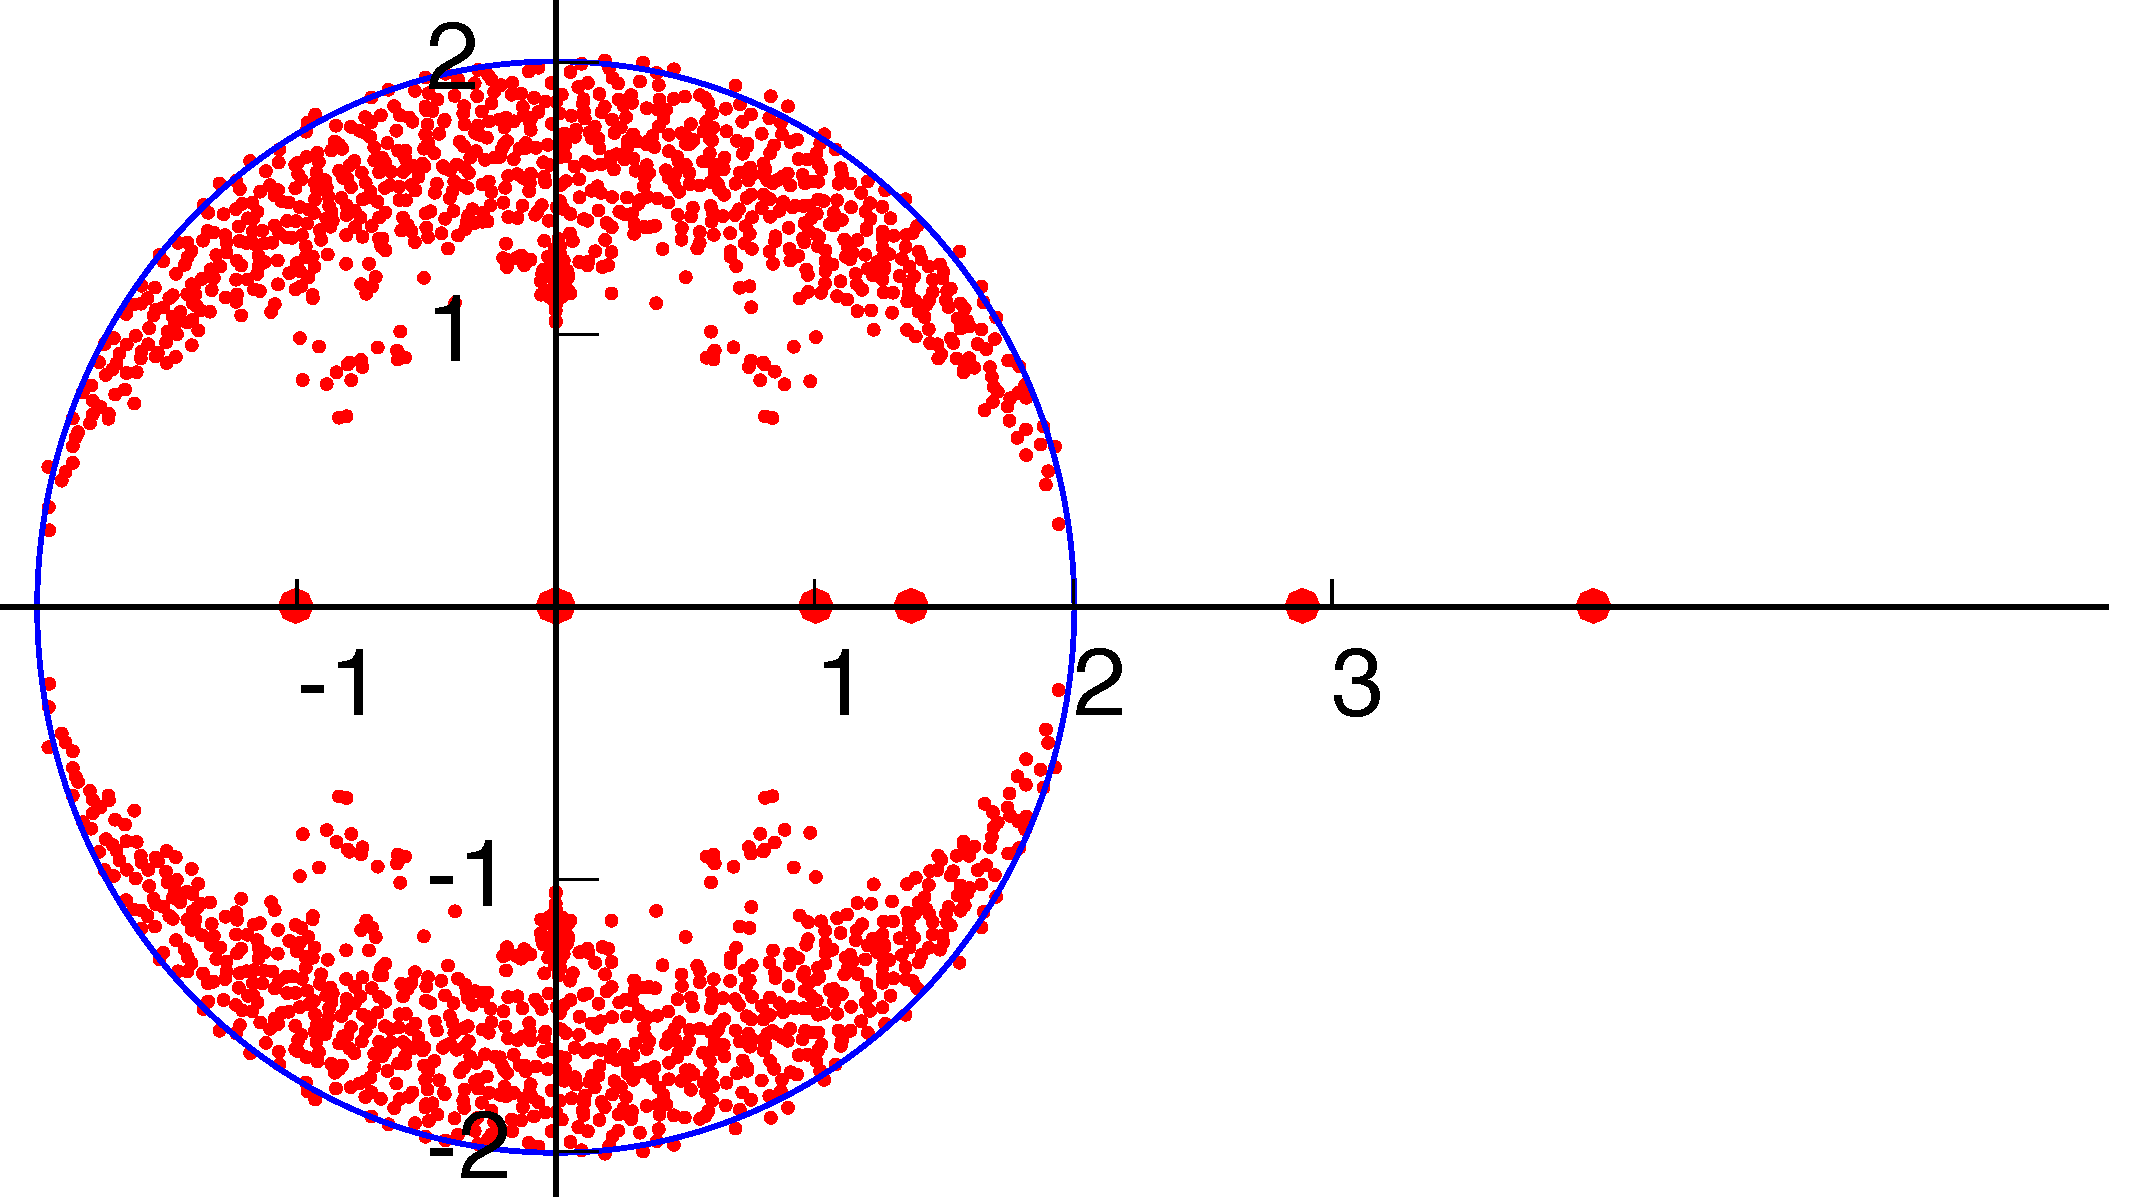
\includegraphics[width=0.5\textwidth]{1000}
	\end{wrapfigure}
	\quad \\[2.5pt]
	Stochastic block model
	\begin{itemize}
		\item $n = 10^4$
		\item $c = 4$
		\item $\cout / \cin = \frac{1}{7}$
	\end{itemize}
	\quad \\[5pt]
	\insfig{AE}
}

\frame{
	\frametitle{Experiments}
	\insfig{EXB1}
	\insfig[0.8]{EXB2}
}

\frame{
	\frametitle{Conclusions} % and Perspectives}
	\begin{itemize}
		\item Comparing to non-backtracking clustering
			\begin{itemize}
				\item $H(r_c)$ is $n\times n$ symmetric, while $B'$ is $2n\times 2n$ non-symmetric
				\item Need to compute $\rho(B)$ to calculate $r_c = \sqrt{\rho(B)}$
					\begin{itemize}
						\item By solving quadratic eigenproblem~(\ref{eq2}) using a SLP algorithm\footnote[frame]{Axel Ruhe (1973). Algorithms for the nonlinear eigenvalue problem. SIAM Journal on
Numerical Analysis, 10(4):674–689.} \vspace{-5pt}
\begin{equation}
	\label{eq2}
	\det{H(\lambda)} = \det{\left[\lambda^2\id-\lambda A+(D-\id)	\right]} = 0 \quad \quad %\quad %\quad
\end{equation}
			\end{itemize}
		\end{itemize}
		\item \vspace{-5pt} Detecting the communities in sparse network
			\begin{itemize}
				\item All the way down to the threshold in SBM
			\end{itemize}
		\item The number of negative eigenvalues indicating the number of clusters
	\end{itemize}
}

\begin{frame}
	\Huge{\centerline{The End}}
\end{frame}

%\begin{thebibliography}{9}
%\bibitem{ClFi07}
%J.~Clark and R.~Fierro, ``Mobile robotic sensors for perimeter detection and
%  tracking,'' \emph{ISA Trans.}, vol.~46, no.~1, pp. 3--13, 2007.
%\end{thebibliography}

\end{spacing}
\end{document}